\def\mytitle{KIIIB}
\def\myauthor{Andreas Moller s042809, David Emil Lemvigh s042809}
\def\affiliation{IMM@DTU}
%==================================================================================================
%   LUKES THESIS TEMPLATE 1.2
%   -------------------------
%   This template is based upon the offcial IMM PhD Thesis template, it is enhanced with a number 
%   of new features and a number of errors have fixed. This template is intended to be complied to 
%   PDF using PDFLATEX and is tested using the MiKTeX 2.9 LaTeX distribution. 
%   It is based on the official DTU-IMM Thesis template by Finn Kuno Christensen in 2009. 
%   -------------------------
%   Last Updated: 04-10-2011
%   Contact: lthhe@imm.dtu.dk
%==================================================================================================
%
%==================================================================================================
% DOCUMENT SETUP
%==================================================================================================
\documentclass[10pt,twoside]{book}                  %Official DTU-IMM Thesis document setup
%
%Set to 'print' for printed version, use 'net' for online version
\def\thesisversion{print} 			
%
%==================================================================================================
% PACKAGES
%==================================================================================================
\usepackage{LukeThesis}                             %Import Thesis base style 
\usepackage{listings}								% Import source listing package
\usepackage{color}
\usepackage[danish]{babel}

\usepackage{amsmath}
\usepackage{amssymb}
\usepackage{graphicx}				% Graphics
%\usepackage[ansinew]{inputenc} 		% UTF8 supprt
%\usepackage[T1]{fontenc}			% Some other characters

\usepackage{hyperref}				% So that \autoref works
\usepackage{url}					% So that \url works

\usepackage{tabulary}				% So we can have tables
\usepackage{booktabs}				% Better tables (aparently)

\usepackage[sort&compress]{natbib} 	% Better bibliography support
\bibpunct{(}{)}{;}{n}{}{,}			% Author-Year fix (apparently)

%\setlength{\parindent}{0pt}			% Sets paragraph indent to zero
%\setlength{\parskip}{7px}			% Adds space between paragraphs
%\setlength{\columnsep}{20px}		% Adds space between coloums

 


%input{PhDMacros}                                   %Thesis specific macros 
%
%==================================================================================================
% THESIS PROPERTIES (Modifiy these fields with your details)
%==================================================================================================
\def\thesisauthor{\myauthor}                     %Author
\def\thesistitle{\mytitle}		         		 %Title
\def\thesishandin{24-Febuary}					          %Submission date (Day-Month}
\def\thesisyear{2012} 							          %Submission year 
\def\thesisnumber{????}  						          %DTU-IMM Serial number (do not include year)
\def\thesisISSN{0000-0000}                          %ISSN number
\def\thesiskeywords{Keywords are, comma separated}  %PDF keywords 
\derivethesisprops                                  %Derive dependent properties

%==================================================================================================
% Source listing properties
%==================================================================================================
\definecolor{dkgreen}{rgb}{0,0.6,0}
\definecolor{gray}{rgb}{0.5,0.5,0.5}
\definecolor{mauve}{rgb}{0.58,0,0.82}

\lstset{ %
  language=Java,                % the language of the code
  basicstyle=\scriptsize,           % the size of the fonts that are used for the code
  numbers=left,                   % where to put the line-numbers
  numberstyle=\scriptsize,          % the size of the fonts that are used for the line-numbers
  stepnumber=1,                   % the step between two line-numbers. If it's 1, each line 
                                  % will be numbered
  numbersep=5pt,                  % how far the line-numbers are from the code
  backgroundcolor=\color{white},      % choose the background color. You must add \usepackage{color}
  showspaces=false,               % show spaces adding particular underscores
  showstringspaces=false,         % underline spaces within strings
  showtabs=false,                 % show tabs within strings adding particular underscores
  frame=single,                   % adds a frame around the code
  rulecolor=\color{black},        % if not set, the frame-color may be changed on line-breaks within not-black text (e.g. commens (green here))
  tabsize=2,                      % sets default tabsize to 2 spaces
  captionpos=b,                   % sets the caption-position to bottom
  breaklines=true,                % sets automatic line breaking
  breakatwhitespace=false,        % sets if automatic breaks should only happen at whitespace
  title=\lstname,                   % show the filename of files included with \lstinputlisting;
                                  % also try caption instead of title
  numberstyle=\tiny\color{gray},        % line number style
  keywordstyle=\color{blue},          % keyword style
  commentstyle=\color{dkgreen},       % comment style
  stringstyle=\color{mauve},         % string literal style
  escapeinside={\%*}{*)},            % if you want to add a comment within your code
  morekeywords={*,...}               % if you want to add more keywords to the set
}



%
%==================================================================================================
% SECTION NUMBERING SETUP
%==================================================================================================
\setcounter{tocdepth}{2}                            %2 adds sections up to subsections
\setcounter{secnumdepth}{3}                         %Subsubsections get a number when this is 3
%
%==================================================================================================
% THESIS STRUCTURE  (Modifiy to include more chapters etc)
%==================================================================================================
\begin{document}
%------------------------                                    
%Pre-frontmatter material
%------------------------
\prefrontmatter
%--------------------
%Frontmatter material
%--------------------
\frontmatter
\pagenumbering{roman}                               %Set frontmatter numbering style
\chapter{Summary (English)}

	The goal of the thesis is to explore the posebillities of a smart house system, with a minimal setup. The goal is to make it as easy as possible for the user, to install and use the system. The system should learn from the user's normal behavior, and eventually be able to copy the user's behavoir and take over control of the home, in a way that also reduces power consumption.
								             %English summary of Thesis
\markboth{}{}                                       %Set headings (left)(right)
\chapter{Summary (Danish)}
\begin{otherlanguage}{danish}

Målet for denne afhandling er at ...

\end{otherlanguage}								             %Danish summary of Thesis
\markboth{}{}                                       %Set headings (left)(right)
\chapter{Preface}

This thesis was prepared at the department of Informatics and Mathematical Modelling at the Technical University of Denmark in fulfilment of the
requirements for acquiring an M.Sc. in Informatics. 

The thesis deals with ... 

The thesis consists of ...
%==================================================================================================
% SIGNATURE AREA
%==================================================================================================
\vspace{20mm}
\begin{center}
	\hspace{20mm} Lyngby, \thesishandin-\thesisyear 
	\vspace{5mm}
	\newline
  %Update signature image file in line below
	
\includegraphics[scale=0.5]{figures/SignatureDummy.jpg}
\end{center}
\begin{flushright}
	\thesisauthor
\end{flushright}
% % % EOF % % %
								             %Preface
\markboth{}{}                                       %Set headings (left)(right)
\chapter{Acknowledgements}

	I would like to thank my....

					             %Acknowledgements
\markboth{}{}                                       %Set headings (left)(right)
%------------------
% Table of contents
%------------------
\newpage\mbox{}\newpage
\chaptermark{Contents}					
\renewcommand{\sectionmark}[1]{\markright{#1}}
\sectionmark{Contents}
\addtolength{\parskip}{-\baselineskip}
\tableofcontents
\addtolength{\parskip}{\baselineskip}
\renewcommand{\sectionmark}[1]{\markright{\thesection\ #1}}
%-------------
% Main content 
%-------------
\mainmatter


\chapter{Introduction}
\label{introduction}

In the recent years we have seen an increase in climate awareness. The subject is gaining more and more media coverage. A survey conducted from 2007 to 2008 by the international research organization Galllup\footnote{International research organization famous for making polls. http:/\slash ww.gallup.com
~\citep{gallup-2009}: http:/\slash www.gallup.com\slash poll\slash 124652\slash awareness-climate-change-threat-vary-region.aspx}, shows that 82\% of americans and 88\% of europeans are very aware of the current climate issues we are facing such as global warming. In the same survey Gallup also concludes that 67\% of americans and 59\% europeans view global warming as a serious threat to them selves and their families~\citep{gallup-2009}.

\chapter{Analysis}
\label{analysis}

The vision for our project is to create an intelligent home control system that requires minimum configuration and installation while providing optimal power saving, and comfort. 

$<$fortsæt fra vision, og introduktion$>$

\section{Smart House Survey}
\label{smarthousesurvey}

\emph{``If I have seen further it is by standing on the shoulders of giants''} -- Isaac Newton

The beginning of any good project starts with a survey of what already exists in the field. Which smart house solutions already exist, and what are their capabilities? What are the industry standards, if any? This section will provide a representative selection of smart house solutions. However, it will not be an exhaustive survey of all smart house solutions.

First we will establish some basic classifications of smart houses, to better compare the different systems. All systems can contain switches, sensors and remote controls, the difference is the functionally they provide, and how they operate.

We distinguish between three types of systems, which are derived from the taxonomies presented in Boguslaw Pilich's Master Thesis ~\citep{Boguslaw} :

~\citep{Boguslaw}: Boguslaw Pilich. Engineering Smart Houses, DTU IMM MSc Thesis Nr. 49\slash 2004

\subsection{Controllable houses}
\label{controllablehouses}

These are the simplest of the smart house solutions. Input devices like switches, remotes and sensors, can be setup to control output devices like appliance and dimmer switches, HVAC (Heating, Ventilation and Air Conditioning), etc. These solution may also include macros, e.g. where a single button may turn off all the lights in the home. 

\subsection{Programmable houses}
\label{programmablehouses}

These solutions incorporate some degree of logical operations, like having motions sensors not turn on the lights, if lux sensors are above a threshold. They may be able to have scheduled task, e.g. turning down the thermostats during stadard work-hours. The behavior of these systems have to be programmed by the manufacturer or the users. Consequetly, changes in user needs require the system to be reprogrammed.

\subsection{Intelligent houses}
\label{intelligenthouses}

In these solutions some form of artificial intelligence or AI is able to control the home. In computer science the term AI is used very loosely. I our case we will define an intelligent house, as a system that is capable of machine learning. That means that the system is capable of evolving behavioral patterns based on empirical data~\citep{wikipedia-machine-learning}. Consequently, the system will over time adapt itself to changes in user needs.

The solutions presented, are some of the most widespread smart house solutions, and represent the three different types of systems: Controllable, Programmable and Intellight houses.

$<$TODO hurtig conclusion om hver løsning, hvad synes vi om dem$>$

\textbf{INSTEON}

INSTEON is a controllable home control system, targeted at private homes. Nodes in the network can communicate using either RF signals or home's existing electrical wiring. A standard array of devices are supported: 

\begin{itemize}
\item Dimmers \& switches

\item HVAC

\item sprinklers

\item motion sensors

\item assorted bridge devices

\end{itemize}

INSTEON supports external application to be run on PC connected through a bridge devices to the network. By this logic it is technically possible to make the system programmable or even intelligent. However no commercial products providing these features currently exists. ~\citep{INSTEON}

INSTEON's solution is fairly widespread in the US, and is a successor to the Redoak X10 system, and is compatable with it's product. It represents what a commercial controllable smart house is capable. It's functionaly very simplistic, but being able to communicate using the home electrical wiring, makes it a very non-intrusive system to install in an existing home. 



\textbf{Clipsal C-Bus}

Clipsal is targeted at large scale home control. The system is install in such prominent buildings as the Sydney Opera house, Wembly Stadium and many more. Nodes communicate over it's own separate wired network, using the C-bus protocol. Each node has it's own microprocessor, which allows for distributed intelligence. Each node can also be individually programmed, and communicate over the shared bus. This allows unconventional devices like motors for stadium roofs and many other devices to be part of the network. 

Clipsal's C-bus represents the flexibility and scalability programmable solutions on the market are able to achieve. It can also be installed in a private home. However, compared to other systems the rquirement of a separate wiring through-out a home can be a disadvantage. ~\citep{CBus}



\textbf{LK IHC}

LK IHC is targeted at private homes. It can be installed with a wired network, or using wireless communication. This solusion tends to be build around simple switches, but with programmable scenarios, e.g. having a switch near the front door and the master bedroom that turns off all lights. It is a modular system, where modules like wireless communication or alarms, can be added to the base installation. 

The basic LK IHC installation is a controllable system. However, the modules can provide programmable functionality to the system, i.e. motion sensors normally control the lights, but if the alarm system is activated, the system calls 911. LK IHC was per 2008 installed in nearly 30\% of newly constructed building in denmark.~\citep{MSsurvey} ~\citep{LK IHC}

\textbf{MIT House\_n}

House\_n differs from the previous systems, as it isn't a finished implementation, but a framework for research projects. There aren't any widespread commercially available intelligent smart house solution on the market, or atleast according to our classification of intelligent. 

House\_n represent one of many smart environment, build by universities around the world. The smart environments are homes for one or more inhabitants, and are part of a living laboratory. The living lab part of House\_n is called PlaceLab, and is a one-bedroom condominium, inhabited by volunteers for varying lengths of time. These homes are designed for multi-disciplinary studies, of people and their pattens and interactions with new technology and smart home environments. Being university run smart homes, the work comming out of these facilities tends to be proof of concepts. ~\citep{MIT House_n}

$<$TODO men fair nok, de er proof on concept, hvilke projekter findes der. Eller hvorfor snakker vi ikke om dem$>$

The projects shown in this survey represent the solutions currently available or in development. There are many different controllable and programmable solution commercially available, with INSTEON, Clipsal C-bus and LK IHC being some of the more widespread representative solutions. INSTEON being a simple controllable solution, Clipsal C-bus and LK IHK are both programmable smart house solutions, but where LK IHC is designed for private homes, the Clipsal C-bus system is better suited for larger buildings. 

MIT's House\_n in this survey represent that truly intelligent smart houses only exists in demonstration environments and as proofs of concept, and are not yet widely available on the commercial market.


One of the main problems with current home control solutions is that installing such a system is rather costly and requires installation and configuration, which is rarely trivial . Some of the more advanced systems on the market, such as the LK IHC, incorporate motion sensors and timers that automatically turn on and off lights or various appliances. These systems will save money over time, but they require extensive configuration or programming in order to function properly.

\section{BIIIB}
\label{biiib}

Of all the qualities mentioned in our vision for the system, power saving is the most important. \textbf{insert data on power consumption of average household} As seen in the survey above, this is an area where most modern home control systems falls short . Most systems are capable of providing only a modest reduction in power consumption, and some even increase the net consumption by adding the cost of running the control system. We want our system to differ from others on this specific aspect. In our system, reducing power consumption is the number one priority.

We will accomplish this by creating a system that focuses on turning off all lights and appliances where they are not needed. $<$what are the alternatives? why do we want to focus on this?$>$There are several advantages to this approach, compared to attempting to reduce the power consumption of active appliances. The main advantage is that it provides the largest reduction in power consumption. Most people remember to turn off the light in the bathroom, when they leave it, but this is far less common for the kitchen, or dining room, and only the most environmentally conscious people would ever turn off the light in the living room when they got to the bathroom. This means that there is a lot of wasted energy in the normal household . 

An other advantage is that it incorporates perfectly with all other power reducing technologies. Bying appliances that use less energy will still give you the same percentage of power reduction as in a normal house. 

This system will also eliminate the common problem of standby mode on many appliances such as tvs or stereos by having the appliance only in standby mode, when the user is likely to turn it on. The rest of the time the appliance is simply turned off.

Our approach to creating a house that is capable of predicting what the users want it to do, is to learn from what the user does and mimic these actions at the right times. To accomplice this, the system must do three things:

\begin{itemize}
\item The system must gather data on the users and their behavior in the house

\item The system must analyze the data in order to build a decision scheme on which it will base its actions

\item The system must be able control the house in real time, based on the decision scheme.

\end{itemize}

Since the system bases its decisions on data gathered on the user, the system is essentially trying to mimic useractions at the right times. The system will have three stages :
$<$must the stages be introduced now? can they wait till the design section$>$
* The untrained stage where the system is running, but it hasn't yet collected enough data to make intelligent decisions. 

\begin{itemize}
\item The learning stage where there's enough data to attempt to manipulate the switches of the home. We call this the learning stage, because it provides us with a unique opportunity for the system to learn from the user. If the system makes a mistake and the user corrects it, e.g., the system turns off the lights and the user turns it back on, we can use that interaction to train our system further. In this case we can see it as the user punishing the system for making a mistake. The system will then adjust its decision scheme. 

\item After the system has been in the learning stage, it will enter its final stage, which we call the evolution stage. Here the system constantly updates its decision scheme with new data both from monitoring the user, and from being punished for its mistakes. In this stage there is a symbioses between the user and the system where the system reacts to the user and vice versa. $<$Som jeg forstår dette, så adskiller det sig ikke fra learning stage. Tekstmæssigt er forskellen, at her er det også brugeren, der ændrer opførsel. Men det har vel ikke noget med systemets udvikling at gøre. - men sandsynligt.$>$

\end{itemize}

\section{Gathering data on the users}
\label{gatheringdataontheusers}

To mimic user actions, the system must first gather information on how the user interacts with the house. Therefore the first question we must answer is: What data should we collect on our users? In order for the system to effectively take over the users direct interactions with the house, we need to know two things. 

\begin{itemize}
\item What action needs to be done?

\item When shall the action be done?

\end{itemize}

The first question can be answered by monitoring the users direct interactions with the house. Since we have limited our system to handle lighting, this means monitoring the users interactions with the light switches.

The second question is a lot more complex. We need to collect data that can help us determine if the conditions are right for performing a specific action. We could of cause quite literally look at the time the action is performed, and then use that as a trigger, but this requires that users follow a very specific schedule.

To get a more detailed picture of when an action is done, we must analyze it relative to what the user is doing at the time. Since we're focussing on lighting this can be done simply by tracking the users movements. Thereby we will determine when an action shall be done based on where the user is, and where he is heading.

Perhaps the most obvious way of accomplishing this is by using cctv cameras. Using visual analysis is the most effective way of monitoring the user, as it will provide us with vast amounts of data on what the user is doing. By for example installing a fisheye camera in every room and use motion tracking on the video data stream, we can determine exactly where the user is, and what he is doing. While this is probably the solution that provides us with the most precise and detailed data, it does have one problem. Installing cameras in every room of the users house is, in out opinion, an unnecessary invasion of the users privacy. Even if the video data is not stored in the system, the presence of cameras will give many people the feeling of being watched in their own homes. 

An other approach would be to use a beacon worn by the user that sends out a digital signal. The system could then use multilateration to pinpoint the exact location of the user. The beacon could be attached to the users keychain, incorporated into his cellphone, or, our personal science fiction favorite, injected under his skin. Like the camera approach this solution also has very high precision in tracking the user through the house. However,besides the point that the user might not always carry his keys or cellphone around, the main issue with this solution is scalability of users. . Even though we limit the system to one user for now , we want a system that can be scaled to accommodate multiple users acting both and autonomously. Having to attach a beacon to every visitor coming into the house is gonna be an annoyance, and without it the house would not react to the visitor at all. 

The solution we chose is to use motion sensors. While this solution does not provide nearly the same precision in determining the users location as using fish eye cameras or multilateration, motion sensors does come with a range of other advantages. Motion sensor is a very cheap solution, compared to installing cctv cameras, and will be far less invasive on the user's privacy. The motion sensor solution will also work for any user in the house, and does not require the user to carry any beacon device like in the multilateration system. 

The system could easily be expanded by several other types of sensors as well. E.g. pressure sensors in the furniture, so the system can determine if there is someone present, even when motion sensors do not register them. There are several other examples of sensor technologies that could be incorporated in the system. Some will be discussed in the section `Future work'. 

For the moment we want to use as few hardware components as possible. There are two reasons for this:

\begin{itemize}
\item We want to keep the system as simple as possible from the consumers perspective. That means a system with as few components as possible.

\item Creating a system that analyses and mimics user behavior will have a lot of unknown variables that are hard to predict no matter how it is implemented. It will therefore be preferable to start out with a system that is stripped down to the bare necessaries and then add components as the need for them arises.

\end{itemize}

We have chosen not to inquire??? any information on the position of the motion sensors in the house.$<$REWRITE, and explain$>$ This means that the system does not know where each sensor is positioned, nor which other sensors are in the same room as it (the sensor og system?). This does make analyzing the data a lot more complicated, but we want to stick with the idea of minimizing the installation and configuration. This way the installation process can be boiled down to putting up the sensors, plugging in the system, and pressing ``Start''.

Choosing to only monitor the light switches and using motion sensors to track the user greatly simplifies the data collection. Both the motion sensors and the switches generate events when they are triggered, and the system should simply store these events in a database. 

An alternative to this is to have the system analyze the data live, which would eliminate the need to store the event data. With this approach we do not have to store the events in the system, which over time could amount to a considerable amount of data. The problem is that if we should choose to modify the algorithms that analyze the data, we would effectively loose everything the system has learned so far. By storing the raw event data we can always recalculate a new decision scheme based on the collected data. This solution leaves us with a lot more options later on. The collection of data must still happen in real time. Since it is very important that the events are recorded exactly when they happen, the system must not stall in this process.

\section{Analyzing the collected data}
\label{analyzingthecollecteddata}

\emph{“If you torture data long enough, it will tell you what you want!”} -Ronald Coase Hvorfra

Now that we have a lot of data on our users interactions with the house, we need to analyze the data in order for our systems AI to act on the collected data. To be more specific: We need to create a decision scheme that the AI can use as a base for its decision making. 

This is the critical part of the system. Collecting data, and acting based on an existing scheme are bot relatively simple tasks, however, designing the scheme to act, based on collected data, is far more complicated.

The purpose of analyzing the data is to find which specific situations that require the system to perform an action. Since the system does not know which sensors are located near which switches, the system will have to learn these relations based on the data collected. The simplest solution would be to have the system learn which switches and which sensors are located in the same room, and then create a ``link'' between them so the motion sensors control the light. This would result in what we have named the silvan\footnote{Danish building material retail-chain. } system. 

The silvan system is basically having a motion sensor turn on the light when triggered, and then have a timer turn off the light if the sensor is not triggered for a set amount of time. The main problem with this kind of system is that if the user does not trigger a motion sensor regularly, the light will turn off when the user is still in the room. This is commonly a problem in a room like the living room, where the user will likely spend an extended amount of time sitting still. This problem can be addressed by extending the light's timeout time. 

However, this brings us to the second problem. If the user is merely passing by a sensor, the light will still be turned on for its full duration. This greatly reduces the effectiveness of the system from a power saving point of view. 

A better solution is to attempt to identify the users behavior leading up to a switch event . Since the system only use motions sensors to track the users movements, these sensor events will form the basis for the data analysis. The system could simply look at what sensor was triggered right before a switch was activated, and the create a link between that sensor and the switch. This, however, would result in a system much like the silvan system described above. 

If we instead look at a series of sensor events leading up to a switch event, we will get a much more complex picture of what the user is doing. Since the switches in the house are located in fixed positions around the house, these movement patterns should repeat themselves relatively often. The movement patterns that lead up to a switch being turned off, will most likely also differ from a pattern leading up to a switch being turned on, since the user will be either entering or exiting a room. Once we have analyzed the data and identified the movement patterns related to a switch event, we need to create a decision scheme that the system can base its decision making on. That means we have to organize the analyzed data in a way so we easily can look up a specific pattern, and see whether it should trigger a switch action.

At first the system will need to gather enough data to make a solid analysis (the untrained stage). The length of this period will vary depending on how the data is analyzed.
Unlike data collection, analyzing the data does not have strict time constraints. Since the decision scheme will be based on data collected over an extended period of time, the system will not benefit from having the decision scheme updated in real time. As a result the time constraints on analyzing the data will be quite loose, and should not pose as a restriction on the system.
$<$reevalueate!$>$

$<$the house should react to the user, and the user to the house$>$

\section{Controlling the house}
\label{controllingthehouse}

After we have collected and analyzed data the the final task is to have the system control the house in real time, using the decision scheme created from the analyzed data. The system must constantly monitor the user and attempt to match his movement pattern to those present in the decision scheme. As with data collection this has to happen in real time so the patterns are not corrupted.

\section{Requirement specification}
\label{requirementspecification}

Based of the analysis above we can now form a requirement specification for the project. The system shall collect data using motion sensors and by monitoring switches. This data should be stored as it is collected and without being manipulated. 

The system should first be in an unlearned stage. In this stage the system should use the collected data to analyze the users movement patterns, leading up to a switch event, in order to create a decision scheme that can help the system mimic the actions of the user . The system should then enter a learning stage, where the system attempts to interact with the switches and learns from the users reactions. $<$shall we remove references to the stages? when does it change state?$>$ Finally the system should enter, and stay in, an evolution stage, where the system constantly learns both from the actions and reactions of the user.
$<$Svært at se, hvad forskellen mellem lærings og evolutionsfasen er. Ud over at systemet konsekvent bliver klogere og klogere? $>$

\chapter{Design}
\label{design}

\begin{itemize}
\item Develop the overall software architecture

\begin{itemize}
\item Identify major system components

\item Specify interactions between system components

\item Specify system components

\begin{itemize}
\item interfaces

\item semantecs

\end{itemize}

\end{itemize}

\item The Design section should allow a skilled programmer to implement the system

\end{itemize}

NOTES:
the system has two steps.
* first it analyzes collected user data. This is one way communication. The user acts and the system listens. this part is done, and have been tested. Training period.
* Now the system evolves by adjusting to the user. The System still collects data, as in step one, but it now interacts with the house, and the user reacts to the system. The system evolves based on the reactions of the user. The system never stops evolving. 

\section{theory}
\label{theory}

\section{Sensor data}
\label{sensordata}

In order to train the system, some sensor data is needed, but how to obtain it? A couple of options are available:

\begin{enumerate}
\item Physical data, setting up wireless motion sensors and switches in a home, and collect the sensor data in a database.
1a A full installation, where the wireless switches are able to turn the light on and off, and by extension also the system.
1b A placebo installation, where the wireless switches doesn't control the light, and merely collect training data.

\item Simulated data, sing a simulator to generate data.

\item Constructed data, manually or algorithmicly generated data.

\end{enumerate}

Looking only at the quality of the data, the best would be to setup an entire house with switches controlling the light, and motion sensors in every room. However installing the system into an existing home would be difficult. The motion sensors and wall socket switches would be fairly easy, but most homes have ceiling with wires in the walls. This means a complete installation of wireless switches would be difficult and costly.
A placebo solusion to the complete installation would be to have wireless wall socket switches next to all the actual switches. By have the users press the placebo switches and the actual switches when they use the light, it's possible to get the training data without having to permanently install the system into the home. It does come with the drawback that it will only be able to generate data for the untrained stage, since the system would not be able to manipulate the actual switches.

People are not robots, and while we are creatures of habit, our movement patterns do not run like clockworks. No matter how well we would generate training data using simulators, algorithms or any other artificial method, there would always be a doubt on how close to actual human behavior it actually is.

We chose to install a placebo system of wireless switches and sensors, to collect training data. This gives us the best quality training data, for the untrained stage of the system, without the expenses of installing operational wireless switches. 

With the training data, we can then use a simulator to evaluate the training stage. In the training stage, there it doesn't take that much data, to evaluate that the system is learning properly. The data from the simulator is good enough to simulate simple movement patterns, to see which lights go on or off, as a simulated user moves from room to room. 

\section{Event patterns}
\label{eventpatterns}

One thing is knowing where the user is, another where the user is headed. By also looking at the preceding interval leading up to an event, it's possible to match that against previously observed patterns, to estimate where the user might be headed.

To determine these pattern we try to make some rules about what to look for. If too long time passes between event, the event are probably not part of the same movement pattern. But what is too long time? 

\section{Zones}
\label{zones}

In many cases to cover an entire room with sensors, the sensors end up overlapping in some areas. This overlapping can be used to increase the precision of the sensors. If two sensors triggers shortly after each other, then the user is in the zone where the two sensors overlap. In cases where multiple sensors triggers at the same time, it can be seen as one zone event.

Take (\autoref{zoneimg}) as an example, of three sensors which overlap a bit, and three paths past the sensors a, b and c. The paths b and c should only be observed as zone events by the system. While path a should look something like 1, zone 1 \& 2, 2, zone 2 \& 3, 3. depending on the cooldown of the sensors each event may be multiple times in the pattern.

\begin{figure}[htbp]
\centering
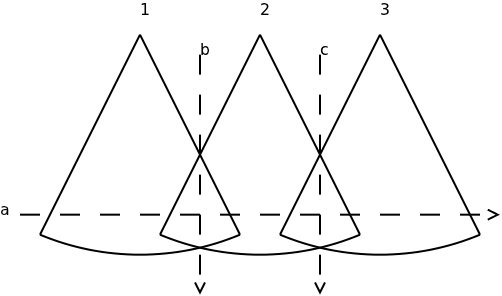
\includegraphics[keepaspectratio,width=\textwidth,height=0.75\textheight]{figures/zone.png}
\caption{Sensors with overlapping zones}
\label{zoneimg}
\end{figure}



\section{Switch and sensor correlation}
\label{switchandsensorcorrelation}

It is beneficial to get a sense of which sensors are near which switches. And we have a lot of statistical data too look at. When a user turns a which on, it most likely because there isn't light where the user intends to be in the immediate future. So it is possible to get an idea of which sensors are near a which, by looking at the interval shortly after a switch is turned on.

$<$TODO maybe talk about that is is less likely that a user will turn on a switch on, and then not enter that room$>$

When flicking a switch off, the user may be leaving the room, or just have entered the room to turn the switch off. Each of the two cases are just as likely as the other, but the sensor events in the interval leaving up to the off event is completely opposite. 

$<$TODO you could possebly look at the interval after it's turned off, and say there are less likely to be in the room, and then try to reduce the correlation for those sensors (NYI)$>$

Based on the statistical data it is possible to generate a table of probability that a sensor is triggered shortly after a switch is turned on, and by extension of that give a idea of wich sensors are in the same room as a switch

\[ P(sensor_i | switch_j , \Delta t) = \frac{\sum 1_{sensor_i} (switch_i, \Delta t) }{\sum switch_j \ events } \]

The indentity function $ 1_{sensor_i} (switch_i, \Delta t) $ is 1 if the sensor is triggered within $\Delta t$ after $switch_j$ is triggered, and is not therefor not counted twice, in the sensor triggeres multiple times after the same switch event.

So to reiterate $ P(sensor_i | switch_j , \Delta t) $ is the probability that $sensor_i)$ fires within $\Delta t$ after $switch_j$ fires.

\begin{table}[htbp]
\begin{minipage}{\linewidth}
\setlength{\tymax}{0.5\linewidth}
\centering
\small
\caption{Correlation table}
\label{ctable}
\begin{tabulary}{\textwidth}{@{}ccccc@{}} \toprule
&sensor 1 $(se_1)$&sensor 2 $(se_1)$&{\ldots}&sensor n $(se_n)$\\
\midrule
switch 1 ($sw_1)$&$P(se_1 | sw_1, \Delta t)$&$P(se_2 | sw_1, \Delta t)$&{\ldots}&$P(se_n | sw_1, \Delta t)$\\
switch 2 ($sw_2)$&$P(se_1 | sw_2, \Delta t)$&$P(se_2 | sw_2, \Delta t)$&{\ldots}&$P(se_n | sw_2, \Delta t)$\\
$\vdots$&$\vdots$&$\vdots$&$\ddots$&$\vdots$\\
switch m ($sw_m)$&$P(se_1 | sw_m, \Delta t)$&$P(se_2 | sw_m, \Delta t)$&{\ldots}&$P(se_n | sw_m, \Delta t)$\\

\bottomrule

\end{tabulary}
\end{minipage}
\end{table}


\chapter{Implementation}
\label{implementation}

\begin{itemize}
\item Description of the system components

\item The implementation section should allow a skilled programmer to maintain the software

\item \textbf{Remember, the most important documentation of the implementation is comments in the code!}

\end{itemize}

\section{Training data collection}
\label{trainingdatacollection}

In order to collect training data, we installed wireless switches and PIR sensors\footnote{Passive infrared sensors.} in a home (\autoref{hellebaekgade}). The placebo switches were placed next to the normal switches controlling the light for each room, in all cases being the switch closest to the entrance. Each room have one or more PIR sensors, averaging 2 per room, with one lest in the restroom and an additional sensor in the living room. When placing the sensors, the system can obviouly only laern from behavoir in areas covered by sensors. So sensors should provide as close to full coverage as possible, with special emphasis on making sure the entrances are covered.

\begin{figure}[htbp]
\centering
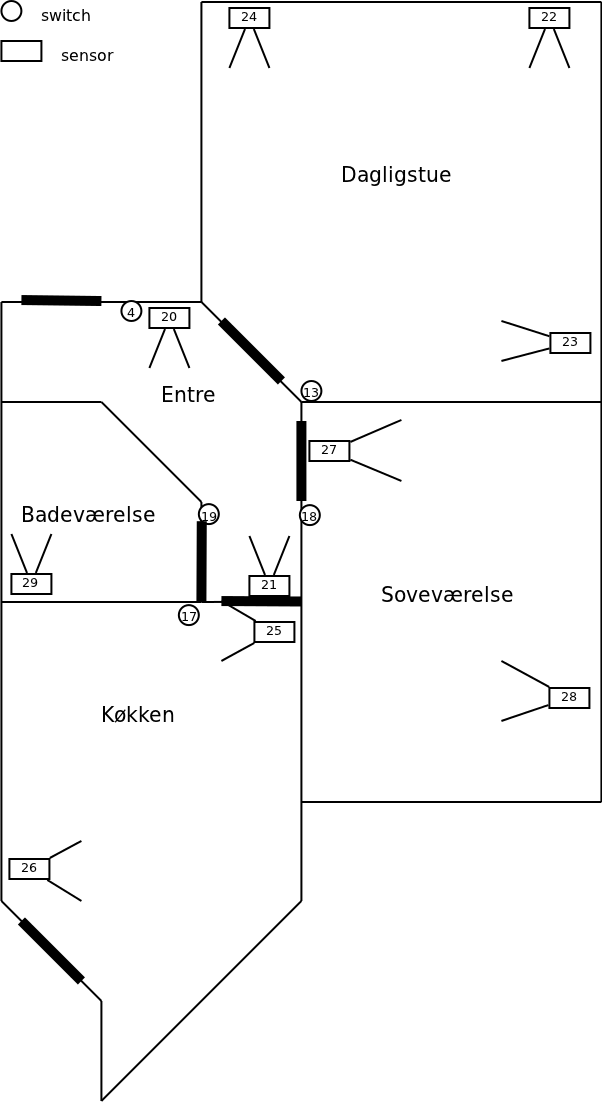
\includegraphics[keepaspectratio,width=\textwidth,height=0.75\textheight]{figures/hellebaekgade3.png}
\caption{Map of the testing environment with sensor and switch locations}
\label{hellebaekgade}
\end{figure}



The wireless nodes we have available communicate using the Zensus Z-Wave protocol. We setup a mini PC with a Z-Wave serial device, and configured all PIR sensor and switches to send notifications to the PC, when they where activated. The PC ran a Z-Wave API, which we added a listener to, so that sensor and switch event was logged to a SQL database.

\begin{table}[htbp]
\begin{minipage}{\linewidth}
\setlength{\tymax}{0.5\linewidth}
\centering
\small
\caption{Database table for sensor events}
\label{sensortable}
\begin{tabulary}{\textwidth}{@{}ll@{}} \toprule
\multicolumn{2}{c}{sensor\_events}\\
\midrule
id&Integer\\
timestamp&Timestamp\\

\bottomrule

\end{tabulary}
\end{minipage}
\end{table}


\begin{table}[htbp]
\begin{minipage}{\linewidth}
\setlength{\tymax}{0.5\linewidth}
\centering
\small
\caption{Database table for switch events}
\label{sensortable}
\begin{tabulary}{\textwidth}{@{}ll@{}} \toprule
\multicolumn{2}{c}{switch\_events}\\
\midrule
id&Integer\\
timestamp&Timestamp\\
status&Boolean\\

\bottomrule

\end{tabulary}
\end{minipage}
\end{table}


\section{Simulator \slash  AI interface}
\label{simulatoraiinterface}

We have a smart house simulator available, which will be extended with an AI module, implementing the features discussed in this report. The simulator is implemented in scala, so an obvious choise would be to implement the AI in scala aswell. However work with the simulator in the initial stages of the project, showed that our programming speed in scala was too slow to get any meaningful amount of work done. The scala language is build upon Java, and both languages compiles to bytecode in \emph{.class} files. A result of that is that Scala and Java interface very easily, and Scala code can invoke Java methods and vice versa. We chose to implement the AI in Java, working in a language we're well-versed in, to increase our productivity and quality of the code.


\section{Decision Matrix}
\label{decisionmatrix}

Antallet af gange den klasse har skiftet navn{\ldots} I've lost count{\ldots}
 - svaret er 4
$<$TODO Andy, you deal with it$>$

\section{Event patterns}
\label{eventpatterns}

To make lookups based on the lastest event pattern, each new sensor event needs to be a matched to see if it's part of a pattern.
As each sensor and switch event is received by the system, a list of the most recent event pattern is maintained in an EventList. 

EventList determines if the lastest event is part of the pattern, and determines if a zone event has occured (if set to use zone events). 

The invariant of the EventList, is that after an event is added, the event list contains the current event patttern. This pattern can then be used to determine if any switches should be turned on or off.

\section{Correlation table}
\label{correlationtable}



\subsection{Correlation statistical generation}
\label{correlationstatisticalgeneration}

Correlation calculates the probability that a sensor is correlated a switch. It scans the database, and looks at the interval just after a switch is triggered. The sensors that triggered in the interval, are counted for that interval, in a way thay they're only counted once per switch event. If a multiple switch event are triggered in the same interval, the sensor events in the overlapping intervals should be counted for each of those switches. Having the number of times each switch is triggered, and each sensors triggeres with the given time interval, it's then calculated the probability that $ sensor_i $ is triggered, given that a $ switch_j $ was turned on atmost $ \Delta t $ ago. This gives the statistical correlation probability table. 

To this the correlation confirmations in the database, is then added. Each row in the database table contains the accululated correlation correction for that switch \slash  sensor pair. The correlation correction is simply added to the correlation based on the statistical data.

The resulting correlation table is allowed to have probabilities above 100\%, which is inteded as destribed in 

\subsection{Correlation correction}
\label{correlationcorrection}

When a switch is turned on, a timer is started for that switch. If a correlated sensor is triggered, it timer is extended. The duration is determined by the correlation between the sensor and the switch, higher correlation gives longer timeouts. If the switch is turned off, the timer is stopped. If the timer runsout a timeoutevent is triggered, and the light is turned off, and a new timer is started, to verify that no manual overrides occur. If the a manual override occurs (e.g. the user turns the switch on again, while the timer is running), the system is ``punished''. The system increases the timeout time, by increasing the correlation between the switch and the first sensor triggered after the switch was turned off. If no manual override occurs, the system was correct in turning off the light, and lowers the timeout time, by reducing the correlation between switch and the last seen sensor before the switch was turned off.

These correlation corrections are stored in a separate table in the database. The correlation use for the timeout is based on both the statistical correlation, and these correlation corrections. The correlation corrections increase or reduce the correlation by 10 percent points. The system allows correlations higher than 100\%, this gives the intended behavoir that a switch may have a longer timeout than what is default.

\section{Timers and timeout}
\label{timersandtimeout}

Timers are implemented in the Timer and Sleeper class. Sleeper is a fairly simple class, it sleeps starts a new thread, sleeps for a given time, then fires a timeout event to a given timeout listener. Timer simply holds a map, where each switch can set a timeout. Timer creates a sleeper object, and puts in the map. The sleepers can then easily be monitored and interrupted if needed. 

To received the timeout events the SmartHouse class implements TimeoutListener. 

\chapter{Evaluation}
\label{evaluation}

\emph{``I have not failed. I've just found 10,000 ways that won't work.''} -- Thomas A. Edison

\emph{``Laughing at our mistakes can lengthen our own life. Laughing at someone else's can shorten it.''} -- Cullen Hightower

\emph{``To err is human--and to blame it on a computer is even more so.''} -- Robert Orben

\begin{itemize}
\item Evaluation should document that the goals have been achieved

\begin{itemize}
\item Functional requirements (i.e., testing)

\item Non-functional requirements (e.g., performance)

\end{itemize}

\item Definition of the evaluation strategy

\begin{itemize}
\item Qualitative-\slash quantitative evaluation

\item Software testing

\begin{itemize}
\item white-box\slash black-box

\item testing levels
*unit testing, integrationg testing, system testing, acceptance testing

\end{itemize}

\end{itemize}

\item summarised output from the evaluation
*output should be explained

\begin{itemize}
\item provisional conclusions should be presented

\end{itemize}

\end{itemize}

\begin{figure}[htbp]
\centering
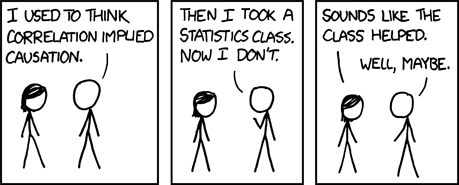
\includegraphics[keepaspectratio,width=\textwidth,height=0.75\textheight]{figures/correlation.png}
\caption{XKCD Correlation}
\label{correlation}
\end{figure}



\section{Correlation}
\label{correlation}

Before evaluating the correlation probability table, some goals should be established.

\begin{itemize}
\item A sensor should have the highest correlation to the switch in the room it's in.

\item Ideally some threshold exists, so that all correlations above the threshold are in the same room, and all other correlations are below the threshold.

\end{itemize}

\begin{table}[htbp]
\begin{minipage}{\linewidth}
\setlength{\tymax}{0.5\linewidth}
\centering
\small
\caption{Correlation table, based on statistical data. $>$ 40\% in bold, 40--20\% in italic.}
\label{ctabledata}
\begin{tabulary}{\textwidth}{@{}rlcccccccccc@{}} \toprule
\multicolumn{2}{c}{Switches}&\multicolumn{10}{c}{Sensors}\\
&&20&21&22&23&24&25&26&27&28&29\\
\multicolumn{2}{c}{}&\multicolumn{2}{c}{Hallway}&\multicolumn{3}{c}{Living room}&\multicolumn{2}{c}{Kitchen}&\multicolumn{2}{c}{Bedroom}&WC\\
\midrule
4&Hallway&\textbf{0.4}&\textbf{0.67}&0&0.2&0.13&0.07&0&0&0.07&0\\
13&Living room&\emph{0.35}&\emph{0.23}&0.12&\emph{0.27}&\textbf{0.42}&0.04&0.04&0.08&0.08&0\\
17&Kitchen&\emph{0.22}&\emph{0.28}&0&0.03&0.17&\emph{0.39}&\textbf{0.58}&0.14&0.03&0.03\\
18&Bedroom&0.1&0.13&0&0&0.03&0.03&0&\textbf{0.57}&\textbf{0.6}&0.03\\
19&WC&\emph{0.29}&\emph{0.29}&0.06&0.09&0.08&0.06&0&0.07&0.03&\textbf{0.75}\\

\bottomrule

\end{tabulary}
\end{minipage}
\end{table}


The correlation table (\autoref{ctabledata}) is based on collected data from the testing environment. The first criteria holds, that all sensors have the highest correlation with the switch in the room they're in.
Most (but not all) the correlation probability between sensors and switches in the same room are above 40\%. All correlations between for switches and sensors not in the same room are below 40\%. Three sensors have correlations lower than 40\% to the switch in the room they're in, and one of them as low as 12\%. Two of the three sensors in the living room, not only have correlations below 40\%, but correlations below those of sensors in the adjecent hallway. As can be seen in the overview of the appartment (\autoref{hellebaekgade}), the sensors 22 and 25 are located in the far end of the rooms from the switch and doorway. Since the calculated correlation probabilities are based on the time interval right after the light is turned on, it makes sense that these sensor, relatively far away from the switches ends up with a lower correlation. 

Sensor 23 is a bit more interesting, since it located fairly close to the doorway. Having one of the authors of this thesis also being the guinea pig running around generating sensor data, gives a unique insight why some sensor patterns look the way they do. Sensor 24 is located by a desk, and 23 next to a sofa. So in this case different user activities triggeres different sensor, in this case sitting on the sofa and watch TV, or go the the desk and work. 

One thing to note is, these are the probabilities based solely on the statistical data, and that correlation corretions would be added onto this schema. So it doesn't perfectly reflect the room \slash  switch + sensor correlations on it's own, though it gives a close approximation

\chapter{Conclusion}
\label{conclusion}

\begin{itemize}
\item summarises all the result of the project

\begin{itemize}
\item what was the problem?

\item what has been achieved?

\end{itemize}

\item presents final conclusions
*summary of provisional conclusions

\begin{itemize}
\item further conclusions drawn from the sum of evidence

\end{itemize}

\item presents directions for future work

\begin{itemize}
\item new problems identified through the project

\item outline the possible evolution curve of the software

\end{itemize}

\end{itemize}

\section{writing good conclusions}
\label{writinggoodconclusions}

\begin{itemize}
\item What was the problem?

\begin{itemize}
\item Remind the reader of the context and project goals

\end{itemize}

\item What was the proposed solution?
-Remind the reader of the proposed solution
 -what was done in the project

\item How did we evaluate the proposed solution?
-Summarize results of indicidual experiments.
 -this inclydes any testing of software in development projects
-Draw conclusions on the endicidual experiments

\item What did we learn?
-Present overall conclusions of the project

\begin{itemize}
\item Outline ideas for future work

\end{itemize}

\end{itemize}

\section{Awesome quotes}
\label{awesomequotes}

lille liste af citater som godt kunne passe ind i rapporten

\emph{I am among those who think that science has great beauty. A scientist in his laboratory is not only a technician: he is also a child placed before natural phenomena which impress him like a fairy tale.} -- Marie Curie

\emph{Good judgment comes from experience, and experience comes from bad judgment.} -- Barry LePatner

\emph{Nothing can be so amusingly arrogant as a young man who has just discovered an old idea and thinks it is his own.} -- Sidney J. Harris

\emph{The more original a discovery, the more obvious it seems afterwards.} -- Arthur Koestler

\begin{thebibliography}{0}

\bibitem{wikipedia-machine-learning}
Wikipedia article on machine learning. http:/\slash en.wikipedia.org\slash wiki\slash Machine\_learning


\bibitem{INSTEON}
INSTEON. http:/\slash www.insteon.net


\bibitem{CBus}
Wipedia article on the Clipsal C-Bus protocol. http:/\slash en.wikipedia.org\slash wiki\slash C-Bus\_(protocol)


\bibitem{MSsurvey}
Mads Ingwar and Soeren Kristian Jensen. IMM Smart House Project: a state of the art survey. 2008.


\bibitem{LK IHC}
Lauritz Knudsens. http:/\slash www.lk.dk


\bibitem{MIT House_n}
MIT House\_n. http:/\slash architecture.mit.edu\slash house\_n\slash placelab.html


\end{thebibliography}

\newpage
\appendix
\section{Source Listings}
%
\subsection{Package: smarthouse}
\subsubsection{SmartHouse.java}
\lstinputlisting[caption=SmartHouse.java]{$KIIIB_HOME/SmartHouse/src/smarthouse/SmartHouse.java}

\subsection{Package: timer}
\subsubsection{Sleeper.java}
\lstinputlisting[caption=Sleeper.java]{$KIIIB_HOME/SmartHouse/src/timer/Sleeper.java}
\subsubsection{Timer.java}
\lstinputlisting[caption=Timer.java]{$KIIIB_HOME/SmartHouse/src/timer/Timer.java}
\subsubsection{TimeoutListener.java}
\lstinputlisting[caption=TimeoutListener.java]{$KIIIB_HOME/SmartHouse/src/timer/TimeoutListener.java}
\subsubsection{TimeoutEvent.java}
\lstinputlisting[caption=TimeoutEvent.java]{$KIIIB_HOME/SmartHouse/src/timer/TimeoutEvent.java}

\subsection{Package: events}
\subsubsection{EventList.java}
\lstinputlisting[caption=EventList.java]{$KIIIB_HOME/SmartHouse/src/events/EventList.java}
\subsubsection{Event.java}
\lstinputlisting[caption=Event.java]{$KIIIB_HOME/SmartHouse/src/events/Event.java}
\subsubsection{SensorEvent.java}
\lstinputlisting[caption=SensorEvent.java]{$KIIIB_HOME/SmartHouse/src/events/SensorEvent.java}
\subsubsection{ZoneEvent.java}
\lstinputlisting[caption=ZoneEvent.java]{$KIIIB_HOME/SmartHouse/src/events/ZoneEvent.java}
\subsubsection{SwitchEvent.java}
\lstinputlisting[caption=SwitchEvent.java]{$KIIIB_HOME/SmartHouse/src/events/SwitchEvent.java}


\subsection{Package: config}
\subsubsection{Config.java}
\lstinputlisting[caption=Config.java]{$KIIIB_HOME/SmartHouse/src/config/Config.java}

\subsection{Package: core}
\subsubsection{Correlation.java}
\lstinputlisting[caption=Correlation.java]{$KIIIB_HOME/SmartHouse/src/core/Correlation.java}
\subsubsection{KeyList.java}
\lstinputlisting[caption=KeyList.java]{$KIIIB_HOME/SmartHouse/src/core/KeyList.java}



\chapter{Source Listings}

\subsection{Package: smarthouse}
\subsubsection{SmartHouse.java}
\lstinputlisting[caption=SmartHouse.java]{$KIIIB_HOME/SmartHouse/src/smarthouse/SmartHouse.java}

\subsection{Package: timer}
\subsubsection{Sleeper.java}
\lstinputlisting[caption=Sleeper.java]{$KIIIB_HOME/SmartHouse/src/timer/Sleeper.java}
\subsubsection{Timer.java}
\lstinputlisting[caption=Timer.java]{$KIIIB_HOME/SmartHouse/src/timer/Timer.java}
\subsubsection{TimeoutListener.java}
\lstinputlisting[caption=TimeoutListener.java]{$KIIIB_HOME/SmartHouse/src/timer/TimeoutListener.java}
\subsubsection{TimeoutEvent.java}
\lstinputlisting[caption=TimeoutEvent.java]{$KIIIB_HOME/SmartHouse/src/timer/TimeoutEvent.java}

\subsection{Package: events}
\subsubsection{EventList.java}
\lstinputlisting[caption=EventList.java]{$KIIIB_HOME/SmartHouse/src/events/EventList.java}
\subsubsection{Event.java}
\lstinputlisting[caption=Event.java]{$KIIIB_HOME/SmartHouse/src/events/Event.java}
\subsubsection{SensorEvent.java}
\lstinputlisting[caption=SensorEvent.java]{$KIIIB_HOME/SmartHouse/src/events/SensorEvent.java}
\subsubsection{ZoneEvent.java}
\lstinputlisting[caption=ZoneEvent.java]{$KIIIB_HOME/SmartHouse/src/events/ZoneEvent.java}
\subsubsection{SwitchEvent.java}
\lstinputlisting[caption=SwitchEvent.java]{$KIIIB_HOME/SmartHouse/src/events/SwitchEvent.java}


\subsection{Package: config}
\subsubsection{Config.java}
\lstinputlisting[caption=Config.java]{$KIIIB_HOME/SmartHouse/src/config/Config.java}

\subsection{Package: core}
\subsubsection{Correlation.java}
\lstinputlisting[caption=Correlation.java]{$KIIIB_HOME/SmartHouse/src/core/Correlation.java}
\subsubsection{KeyList.java}
\lstinputlisting[caption=KeyList.java]{$KIIIB_HOME/SmartHouse/src/core/KeyList.java}



\chapter{Testing}

\section{Source Listings}
\subsection{UnitTests.java}
\lstinputlisting[caption=UnitTests.java]{$KIIIB_HOME/SmartHouse/tests/events/UnitTests.java}

\section{DecisionMatrix dumps}

\subsection{Pattern length 2, without zones}
\lstinputlisting[language=XML, caption=EventList.java]{dump/dump-2-false.txt}

\subsection{Pattern length 2, with zones}
\lstinputlisting[language=XML, caption=EventList.java]{dump/dump-2-true.txt}

\subsection{Pattern length 3, without zones}
\lstinputlisting[language=XML, caption=EventList.java]{dump/dump-3-false.txt}

\subsection{Pattern length 4, without zones}
\lstinputlisting[language=XML, caption=EventList.java]{dump/dump-3-true.txt}

\end{document}
% % % EOF % % %


\end{document}
